\documentclass{article}
\usepackage{icmc,amsmath}
\usepackage{graphicx}
\usepackage{url}
\usepackage[utf8x]{inputenc}
\usepackage[english]{babel}
\usepackage{color}
\usepackage[htt]{hyphenat}

\title{Rameau: A System for Automatic Harmonic Analysis}

\oneauthor
  {Pedro Kröger, Alexandre Passos, Marcos Sampaio}
  {Genos---Computer Music Research Group\\ School of Music
   \\ Federal University of Bahia, Brazil \\
  \url{pedro.kroger@gmail.com}, \url{alexandre.tp@gmail.com}, \url{mdsmus@gmail.com}}

\newcounter{notacounter}

\newcommand{\nota}[1]{
  \addtocounter{notacounter}{1}
  \textcolor{red}{[nota \arabic{notacounter}: #1]}
}


\begin{document}
\maketitle

\begin{abstract}
%The abstract should be placed at the top left column and should contain
%about 150-200 words.

\end{abstract}

\section{Introduction}
\label{sec:introduction}

In music, harmonic analysis is the study of vertical sonorities and it
connections and is paramount to the understanding of tonal
compositions. The analyst can find the root of chords, label
sonorities with proper chords names (such as ``A minor''), and
identify the relationship between chords using roman numerals.

Harmonic analysis by computer is an important, challenging, and
interesting computer music research topic. It is challenging because
the musical material has a large variety of information such as
timber, notes, rhythm, dynamics, harmony, and by the fact that music is
not a linear process, unlike image \cite{mouton95:numeric}. The
harmonic changes in a choral texture, where usually all notes in all
voices begin and finish at the same time, are obvious. However, very
often chords can be arppeggiated, incomplete, and intertwined with
non-harmonic tones. These things contribute to increase considerably
the complexity for analysis \cite{pardo00:automated}. 

There are many practical applications for automatic music analysis,
among them arranging, detection of possible logical mistakes in
scores, database search, automatic accompaniment generation, and
statistical analysis of musical styles for automated composition
\cite{pardo02:algorithms,temperley99:modeling}. Computer-based
harmonic analysis is important because it can bring new insights in
music theory, in the same way the use of computer in vision and
problem solving has brought new insights in these areas
\cite{temperley99:modeling}.

Until now a single framework that allows the comparison between
different algorithms and analysis results has not been developed.
Pardo and Birmingham state that ``no researchers have published
statistical performance results on a system designed to analyze tonal
music'' \cite{pardo02:algorithms} before their paper. This lack of
data in literature makes it difficult to compare different systems.
Also, there aren't standard benchmarks to compare different algorithms
and analysis results. In fact, only Pardo and Birmingham
\cite{pardo00:automated} and Barthèlemy and Bonardi
\cite{barthelemy01:figured} published specific comparisons between
different analysis results. Pardo and Birmingham compare their results
with Temperley and Sleator's \cite{temperley99:modeling} while
Barthèlemy compares his model against Maxwell's, Pardo and
Birmingham's, and Temperley and Sleator's
\cite{maxwell92:expert,temperley96:algorithm,pardo99:automated}.
However, these comparisons are based on results published in papers
and not from direct implementations. That means that only the examples
published by the authors can be compared.

\nota{terminar} In this paper we will present Rameau, a framework for
automatic harmonic analysis of Western tonal music. Our main goal in
building this framework is to allow an easy comparison between
algorithms and results. We also present an evaluation of ten
algorithms using a corpus of 140 Bach Chorales from the
Riemenschneider edition. Section \ref{sec:system} describes Rameau in
more details, section \ref{sec:problem} lists the problems related to
harmonic analysis, section \ref{sec:analysis-results} analyses the
results obtained, and section \ref{sec:concl-future-work} .......

\section{The problem of automated harmonic analysis}
\label{sec:problem}

The problem of automated harmonic analysis might be understood by
dividing it into four sub-problems. 

The first problem is in the system's input format. If sharps and flats
are grouped together the program may have problems in places where
enharmonic information is important. Most systems either ignore this
problem or develop a pitch speller \cite{temperley99:modeling}. To our
knowledge no harmonic analysis software currently uses an input format
that preserves enharmonic information.

The second problem is determining what are the vertical sonorities in
a piece of music and grouping these sonorities into harmonically
significant segments, or chord-spans. This is called the segmentation
problem. Most of the difficulty of segmenting is due to the number of
possible segmentations of a piece being roughly an exponential
function of its length \cite{pardo02:algorithms}.

The third problem is labeling segments with chord names. Not every
segment forms a chord, though - some will consist solely of non-chord
tones and other melodic clues. Labeling a segment with a chord might
require contextual information, which complicates the matter a bit,
difficulting local decisions. Still, over 80\% of accuracy is possible
ignoring context (see section \ref{sec:analysis-results}).

The last problem is finding the key of the piece and assigning a tonal
function to each chord.

\section{Numeric codification for tonal music}
\label{sec:codificacao-jamary}

Probably the pitch-class notation, or some variation such as MIDI, is
the most used way of to numerically represent pitch. The main problem
with this notation is the loss of enharmonic spelling. In this section
we will revise three notations created independently by Brinkman,
Hewlett, and Oliveira \cite{brinkman86:_binom_repres_of_pitch_for,
  hewlett92:base40, oliveira01:codificacao} to address this problem.
For simplicity we will refer to them as binomial, base-40, and
base-96, respectively.

Notes in the binomial notation are represented as tuples in the form
of \texttt{<pc,nc>} where \texttt{pc} stands for pitch-class and
\texttt{nc} for note-class. Note-class is a modulo 7 notation system
that represents numerically each note name (A, B, C, D, E, F, G) from
0 to 6. 0 represents any C, with or without accidentals, 1 represents
any D, with or without accidentals, and so on. For example, C$\sharp$
is represented as \texttt{<1,0>}, D$\flat$ as \texttt{<1,1>}, and Cb
as <11,0>. In this last example 11 represents the pich-class of the
note and 0 indicates how it will be spelled. The binomial notation
also allows a packaged representation using only single numbers, where
the pitch-class is multiplied by 10 and added to the note-class. For
example, C$\sharp$ becomes 10 and D$\flat$ 11.

Unlike the binomial notation, the base-40 notation uses only single
numbers. The octave is divided linearly in 40 notes from C$\flat\flat$
to B$\sharp\sharp$. Table \ref{tab:base40} shows a few notes in this
system.

\begin{table}
  \centering
  \begin{tabular}{l|l}
    note & code \\
    \hline
    c$\flat\flat$ & 1 \\
    c$\flat$ & 2 \\
    c & 3 \\
    c$\sharp$ & 4 \\
    c$\sharp\sharp$ & 5 \\
    -- & 6 \\
  \end{tabular}
  \caption{A few notes in the base-40 notation}
  \label{tab:base40}
\end{table}

The base-96 notation is simple, elegant, and overcomes a few
shortcommings in both the binomial and base-40 notations. Since the
original publication of the base-96 notation is available only in
Portuguese, we will describe it here, comparing with the other
two.

The base-96 also is a single number notation. It has all the
advantagens of the base-40 notation with a few advantagens. Table
\ref{tab:jama-notas} shows how notes are encoded. In this notation the
intervals are invariant under most transformations, such as inversion,
transposition, etc. Table \ref{tab:jama-intervalos} shows the coding
for the intervals. In this table the first column indicates the
interval name; p, M, m, d, A for perfect, major, minor, diminished,
and augmented, respectively. The letters before d and A indicate the
quantity of the interval. For instance, tA is triple-augmented.

\begin{table}
  \centering
  \begin{tabular}{l|lllllll}
               & c & d& e& f& g& a& b \\
    \hline
    7$\flat$   &   & 7&21&  &  &62&76 \\
    6$\flat$   & 90& 8&22&35&49&63&77 \\
    5$\flat$   & 91& 9&23&36&50&64&78 \\
    4$\flat$   & 92&10&24&37&51&65&79 \\
    3$\flat$   & 93&11&25&38&52&66&80 \\
    2$\flat$   & 94&12&26&39&53&67&81 \\
    $\flat$    & 95&13&27&40&54&68&82 \\
    $\natural$ &  0&14&28&41&55&69&83 \\
    $\sharp$   &  1&15&29&42&56&70&84 \\
    2$\sharp$  &  2&16&30&43&57&71&85 \\
    3$\sharp$  &  3&17&31&44&58&72&86 \\
    4$\sharp$  &  4&18&32&45&59&73&87 \\
    5$\sharp$  &  5&19&33&46&60&74&88 \\
    6$\sharp$  &  6&20&34&47&61&75&89 \\
    7$\sharp$  &   &  &  &48&  &  &   \\
  \end{tabular}
  \caption{Notes in the base-96 notation}
  \label{tab:jama-notas}
\end{table}

\begin{table}
  \centering
  \begin{tabular}{l|llllllll}
    & 1$^{st}$& 2$^{nd}$& 3$^{rd}$& 4$^{th}$& 5$^{th}$& 6$^{th}$& 7$^{th}$& 8$^{th}$ \\
    \hline
    sd  &  & 7&21&35&49&62&76&90 \\
    qd  &  & 8&22&36&50&63&77&91 \\
    qd  &  & 9&23&37&51&64&77&92 \\
    td  &  &10&24&38&52&65&78&93 \\
    dd  &  &11&25&39&53&66&79&94 \\
    d   &  &12&26&40&54&67&80&95 \\
    m   &  &13&27&  &  &68&82&   \\
    P   & 0&  &  &41&55&  &  &96 \\
    M   &  &14&28&  &  &69&83&   \\
    A   & 1&15&29&42&56&70&84&   \\
    dA  & 2&16&30&43&57&71&85&   \\
    tA  & 3&17&31&44&58&72&86&   \\
    qA  & 4&18&32&45&59&73&87&   \\
    qA  & 5&19&33&46&60&74&88&   \\
    sA  & 6&20&34&47&61&75&89&   \\
    oA  &  &  &  &48&  &  &  &   
  \end{tabular}
  \caption{Invervals in base-96 notation}
  \label{tab:jama-intervalos}
\end{table}

The base-96 notation works for up to seven flats and sharps, which is
more than enough for tonal music. This system is compatible with the
pitch-class system (modulo 12): in the base-96 notation G = 55, and
the result of 55 mod 12 is 7, representing G in the pitch-class
notation. 

The problem with the base-40 notation is that it only works up to two
accidentals. For example, the interval between C$\flat\flat$ and
C$\sharp\sharp$ (a quadruple augmented unison) has the same value (6)
as diminished second. On the other hand, in the base-96 notation this
interval can be correctly computed.

The main problem with the binomial notation is that operations that
are (and should be) simple become complex. In both base-40 and base-96
notations, transposition is as simple adding an index to a note, while
in the binomial system it has to use two different operations (mod and
div) besides the addition. Its packaged representation is supposed to
simplify things, but as an example, transposition become something
like:

\begin{verbatim}
10 ((a div 10 + B div 10) mod 12)
 + ((a mod 10 + B div 10) mod 7)
\end{verbatim}

To do anything non-trivial, like interval-class vectors, yet extra
work has to be done, increasing complexity.

\nota{falar em algum lugar porque nao usa codificação tonal}

For these reasons we have adopted the base-96 codification, although
no algorithm at present makes direct use of it. We believe it is a
very nice form of describing tonal music numerically and it should be
more known among researches and developers.

\section{The Rameau Framework}
\label{sec:system}

To properly study, understand and compare algorithms for automated
harmonic analysis we have designed and implemented a framework,
Rameau, that should enable us to

\begin{enumerate}
\item compare results precisely and repeatably with human analysis of
  a large corpus of music;
\item allow algorithms to access detailed information in the input score,
  such as enharmonic differences, meter, etc; and
\item easily develop new algorithms, test existing ones, and compare
  precisely the results.
\end{enumerate}

Reimplementing existing algorithms in Rameau allows us to easily
evaluate their accuracy, study their errors and compare them with our
baseline techniques. We are unaware of research comparing different
approaches for harmonic analysis, in the manner of reference
\cite{gomez.herrera:tonality}.

Rameau is written in Common Lisp and runs on the Steel Bank Common
Lisp \cite{team07:_sbcl} compiler on the GNU/Linux operating
system. Rameau also runs on windows (it may run on MacOS, but that was
not tested) and is portable enough to be compiled with CMUCL
\cite{maclachlan06:_cmucl_users_manual} and Clisp
\cite{haible07:_clisp}.

\subsection{Architecture}
\label{sec:architecture-and-api}

The architecture of the Rameau framework is simple. First, a score is
parsed (our parser is written using Cl-Yacc
\cite{chroboczek:_cl_yacc_manual} and Cl-Lexer
\cite{parker:_lexer_packag}) into a list of notes, which is then split
into a list of sonorities. Then, these sonorities are sent to each
algorithm for analysis. The analysis results and their comparison with
the answer sheets are then output either textually or as an annotated
score, as in figures \ref{fig:coral-12} and \ref{fig:coral-54}.

The algorithms used for analysis are implemented using a very simple
Common Lisp API. To implement one it is enough to place a lisp file in
a special directory and call the \texttt{register-algorithm} function
inside that file, specifying the algorithm's name, an analysis
function and a comparison function as parameters. The input to the
analysis function is a list of sonorities. In Rameau, sonorities are
lists of notes, each note specifying its onset time, duration, octave
and pitch. The output is a list of either chords or non-chord tones,
one for each input sonority. Chords are structures possibly having a
fundamental, a mode, a seventh, a bass, and other additions. The
framework provides a few possible comparison functions for easy
usage.

We have currently implemented using this API 
\begin{enumerate}
\item a subset of the algorithm described in \cite{pardo02:algorithms}
  (ignoring, for now, segmentation), 
\item a port (work-in-progress) of the algorithm described in
  \cite{temperley99:modeling}, 
\item four neural networks (using the Fann \cite{nissen:fann}
  library) roughly similiar to some described in
  \cite{tsui02:_harmon_analy_using_neural_networ}, and
\item four decision trees modeled after the neural networks (using code
  from \cite{Mitchell:1997:ML}).
\end{enumerate}

Rameau's source code is publicly available, under a GNU GPL
\cite{fsf:gpl} license in a git \cite{baudis:_git_users_manual}
repository at \url{genos.mus.br/repos/rameau.git} and for
visualization at \url{git.genos.mus.br/?p=rameau.git}.

\subsection{The interface}
\label{sec:analysis-output}

Rameau is basically a command line program, although a GUI version is
planned. The user can select the chorales he or she wants to have
analyzed and specify the algorithms for the analysis. The output shows
a table with the partition number, the correct analysis from each
sonority (take from the answer sheet) and the analysis output for
each chosen algorithm. The nice thing about this output is that it
can be further processed using regular unix tools such as grep, awk,
and sed.

To simplify reading for humans, rameau can output a score with the
chorale and the analysis from each algorithm chosen. The music
notation program LilyPond is used to render the score.

Figure \ref{fig:coral-12} shows the result of the analysis of the
first phrase of chorale \#12. The first line shows the partition
number, the last line the expected answer, and the lines in between
the analysis results for the chosen algorithms. The output score shows
incorrect analysis in bold italic. Non-chord tones are notated as
``—''. It is important to remember that while some algorithms identify
whole chords, others identify only the root.

\subsection{Test Corpus}
\label{sec:test-corpus}

We are building a corpus of analyzed and digitalized Bach chorales to
use as training and test data. Bach chorales were chosen because:

\begin{enumerate}
\item they are easily analyzed. For example, the segmentation problem in
them consists simply of determining the sonorities.
\item Their chord density is high - there are many more chords per
  measure than in a symphony, for example.
\item They are canonical examples of tonal harmony.
\item There are 371 on the Riemenschneider edition, more than
  enough to train our algorithms and get precise error analysis.
\item Their texture is simple and constant. It consists basically of
  four voices forming simple triads and tetrads.
\end{enumerate}

We have already analyzed 140 of them and plan on completing this task
soon. The chorales are stored in a subset of the GNU Lilypond
\cite{nienhuys:lilypond} format, from which we generate MIDI files and
typeset scores, possibly annotated with analysis results (both by
human and by computer).

When the chorales are fully analysed we plan on incorporating the
Kostka-Payne \cite{kostka03:tonal} corpus, Beethoven sonatas, Bach
cello suites and other pieces.

\subsection{The answer sheet format}
\label{sec:formato-dos-acordes}

The results of human analysis performed on the chorales are stored in
a simple, flexible text format, designed to

\begin{enumerate}
\item be as close as possible to usual popular notation,
\item represent inherent ambiguities in chord, and
\item single out sonorities that do not constitute chords, instead
  having melodic functions on the piece.
\end{enumerate}

The first four sonorities of the answer sheet for Bach's chorale \#1
``Aus meines Herzens Grunde'', for example, are stored as \texttt{G G
  C/E (C7+/E [b])}. Each chord symbols represents a sonority. Chords
in parenthesis represent possible interpretations of a single
sonority. Notes in brackets are non-chord tones, marking sonorities
that do not constitute chords.

This information is then used as answer sheets and training data on the
many algorithms implemented in our system.

\section{Comparison with similar works}
\label{sec:differences-from-similar-software}

\nota{fazer uma revisao maior}

We only had access to one similar system, Temperley and Sleator's
Melisma \cite{temperley99:modeling}. The output of the system is
complex, with many not clearly delimited columns that can't be
processed in isolation. Interpreting which notes are chord changes is
difficult even for a human. Therefore, we have been unable to
reproduce their claimed accuracy with their implementation. Our
reimplementation isn't currently able to process every chorale (the
algorithm is brittle and needs tuning in not clearly defined ways),
but averages around 60\% on the ones it does handle.

Pardo and Birmingham's HarmAn \cite{pardo99:automated} system isn't
publicly avaliable on the internet, so we haven't been able to test it
directly. Their algorithm, however, is reimplemented in Rameau, and it
behaves precisely as described in the article.

Our main issues with both systems are their ignorance, by design, of
non-chord tones and their lack of automated test suites for their
algorithms. This difficults a clear evaluation of their merits and
flaws.

\section{Preliminary results}
\label{sec:analysis-results}

\nota{escrever introdução basica}

\subsection{Pardo and Birmingham's Algorithm}
\label{sec:pardo-birmingham}

The algorithm described in \cite{pardo99:automated} has some
interesting properties. It handles most simple examples of tonal
harmony really well, but has no clear notion, by design, of non-chord
tones, augmented chords and other possible analysis. We
have found no need, as of yet, of implementing the segmentation
algorithm, since segmentation is trivial in Bach Chorales.

The current accuracy is $66 \pm 9\%$.


\subsection{Neural Networks}
\label{sec:neural-nets}

Neural networks are a tool to perform non-linear statistical data
modeling that works by having artificial ``neurons'' exchange
information. There are many varieties of neural networks, each being
useful for a certain type of problem. Our networks are all multilayer
feedforward neural networks, with one hidden layer each. This is the
standard model for pattern recognition \cite{russell02:aima}.

A neural network is made of connected neurons. Each neuron receives
signals from other neurons, processes them in a simple manner and
forwards them to yet other neurons, as in figure \ref{fig:neuron}. In
a feedforward neural network, these signals flow linearly from input
neurons to output neurons. Our networks are layered feedforward neural
networks, in which the neurons are arranged in layers, as in figure
\ref{fig:simple-net-diagram}. Each neuron receives information from
all neurons in the layer preceding it and forwards information to all
neurons in the next layers. The first layer, the input layer, receives
the input to the neural network as information, and the output layer
emits the neural network's outputs. One hidden layer between the input
and output layers is enough to represent every continuous function
with arbitrarily small error \cite{russell02:aima}. How each
individual neuron will process its input is determined by training,
usually with the backpropagation algorithm or a variant of it.


\begin{figure}
  \includegraphics[scale=0.35]{neuron}
  \caption{A single neuron in a neural network}
  \label{fig:neuron}
\end{figure}

\begin{figure}
  \includegraphics[]{neural-networks}
  \caption{The Simple-net}
  \label{fig:simple-net-diagram}
\end{figure}


We, in Rameau, have currently implemented four neural-network-based
algorithms for harmonic analysis, basing our approaches on
\cite{tsui02:_harmon_analy_using_neural_networ}. The input of our
simplest algorithm, \texttt{Simple\hyp{}net}, is a sonority's pitch
count, or how many times each pitch class sounds in it. As output, the
network activates the neuron representing the fundamental for that
sonority (or does nothing, if the sonority does not form a chord).
Figure \ref{fig:simple-net-diagram} shows its connections and labels.
To study the effect of contextual information we have also implemented
\texttt{Context-net}, differing from the \texttt{Simple\hyp{}net} only
by also looking at the pitch counts two preceding and one following
sonoritie. Their performances are equivalent, so perhaps the
contextual information necessary for harmonic analysis is not easily
inferrable from pitch counts. The two other neural networks,
\texttt{Chord-net} and \texttt{Mode-net}, also determine a chord's
mode and its seventh. \texttt{Chord-net}'s input is the same as
\texttt{Sim\-ple\--net}'s, while and \texttt{Mode-net} also sees the
results of \texttt{Context-net}'s analysis for each sonority.

The performance of each neural network depends heavily on the number
of hidden units it uses. Too few units and the network hasn't got
enough memory to learn enough harmonic patterns. Too many, and the
network faces the risk of overfitting. Overfitting happens when the
neural network has too much memory, so it starts inferring inexistent
patterns from noise in the training data. This is similar to a
superstitious person's belief that some things bring ``good luck'' or
``bad luck'', according to \cite{white95:superstitious}.

The ideal number of hidden units in a neural network has to be
determined experimentally. The experiments for each of our networks
can be seen figures \ref{fig:simple-net}, \ref{fig:context-net},
\ref{fig:chord-net}, and \ref{fig:mode-net}. The chosen values were 12
units for \texttt{Sim\-ple\--net}, 24 for \texttt{Context-net}, 55 for
\texttt{Chord-net} and 50 for \texttt{Mode-net}.

Our current accuracies for these algorithms are $88\pm 8\%$ for
\texttt{Simple-net}, $87 \pm 8\%$ for \texttt{Context-net}, $83 \pm
8\%$ for \texttt{Chord-net} and $83 \pm 8\%$ for \texttt{Mode-net}.

\begin{figure}
  \includegraphics[scale=0.35,angle=270]{dados-simple-net}
  \caption{Accuracy versus number of hidden nodes in the simple-net}
  \label{fig:simple-net}
\end{figure}

\begin{figure}
  \includegraphics[scale=0.35,angle=270]{dados-context-net}
  \caption{Accuracy versus number of hidden nodes in the context-net}
  \label{fig:context-net}
\end{figure}

\begin{figure}
  \includegraphics[scale=0.35,angle=270]{dados-chord-net}
  \caption{Accuracy versus number of hidden nodes in the chord-net}
  \label{fig:chord-net}
\end{figure}

\begin{figure}
  \includegraphics[scale=0.35,angle=270]{dados-mode-net}
  \caption{Accuracy versus number of hidden nodes in the mode-net}
  \label{fig:mode-net}
\end{figure}

\subsection{Decision Trees}
\label{sec:decision-trees}

Decision trees are useful data modeling tools, with many uses in the
machine learning community \cite{Mitchell:1997:ML,
  russell02:aima}. They are most useful when trying to extract
meaningful patterns from data in a human-readable way. We have built
four decision trees that perform harmonic analysis, each mirroring one
of the neural networks. Our original intention was analysing the rules
generated by the trees to better understand harmonic analysis, but we
have found, looking at their shapes, that the trees haven't
generalized beyond memorizing their inputs. \texttt{Chord-tree}, for example,
doesn't learn the distinction between major and minor modes clearly,
misclassifying most minor chords as major (see section
\ref{sec:common-errors}). \texttt{Mode-tree} only overcomes this by using a
two-step process: first a sonority's fundamental is determined by
\texttt{Simple-tree}, then the sonority is transposed to a normalized
format (the bass is always pitch class 0) and then \texttt{Mode-net}
is applied. This effectively reduces the input space, limiting the
effects of poor generalization.

Our current accuracies for the decision-tree based algorithms are $82
\pm 8\%$ for \texttt{Simple-tree}, $76 \pm 9\%$ for
\texttt{Context-tree}, $77 \pm 10\%$ for \texttt{Mode-tree} and $50
\pm 11$ for \texttt{Chord-tree}.

\subsection{Training set size}

The effect training set size on the accuracy of the neural networks
and decision trees can be seen in figure
\ref{fig:treinamento-corais}. One chorale is enough information for
\texttt{Simple-net}, and most decision-tree algorithms need far more
chorales than their neural-network counterparts to perform similarly,
due to their lower generalization performance.

\begin{figure}
  \includegraphics[scale=0.35,angle=270]{treinamento-corais}
  \caption{Accuracy versus amount of training data per algorithm}
  \label{fig:treinamento-corais}
\end{figure}


\subsection{Common Errors}
\label{sec:common-errors}

\nota{traduzir}

Most analysis errors on our corpus are misrecognized non-chord tones
(58\%), wrong fundamental (24\%) and correct fundamental but wrong mode
(19\%). This last error is the most interesting in evaluating the
accuracy of the algorithms.

Chords analysed with the correct fundamental but incorrect mode can be
classified by which modes are more frequently mistaken for others. The
cateagory with most errors is minor chords labeled as major chords,
with 1550 instances, and the least frequent is incorrectly labeled
major tetrads, with 41 instances.

Os erros de análise cometidos pelos algoritmos nos 140 corais\
analisados envolvem principalmente notas melódicas (58\%), acordes com
tônicas diferentes (24\%) e acordes com tônicas semelhantes, mas de
tipos diferentes (19\%), como por exemplo A maior e A menor. A
interpretação deste último tipo de erro é a mais útil para a avaliação
do funcionamento dos algoritmos.

Acordes de mesma tônica e tipos diferentes podem ser divididos em
categorias a partir do resultado esperado. A categoria com maior
número de erros é a de acordes menores analisados como maiores, com
1550 ocorrências, e a de menor número é a de tétrades maiores, com 41
ocorrências. A Chord tree tem alto índice de erros em quase todas as
categorias, especialmente nas tríades menores. A tabela
\ref{tab:common-errors} contém alguns desses dados, com o valor
percentual de cada algoritmo em cada categoria em função do total de
erros de cada algoritmo.

A figura \ref{fig:coral-54} mostra um excerto de um coral analisado
pelos algoritmos e ilustra todos esses erros. As partições 48 e 49
ilustram notas melódicas analisadas como acordes. A partição 50 contém
uma tétrade menor que é analisada por 5 algoritmos como acorde com
tônica diferente do esperado, por 3 algoritmos como tônica correta e
tríade maior, por um como tríade menor. Neste caso apenas um algoritmo
acerta a análise.

\begin{table}
  \centering
  \begin{tabular}{l|r@{}p{.001cm}r@{}p{.001cm}r@{}p{.001cm}r@{}p{.001cm}r@{}p{.001cm}r@{}p{.001cm}r@{}p{.001cm}}
                 &   °&&  °7&&  ø7&&   m&&  m7&&   M&&  M7 &\\
    \hline
    Pardo-Birm   & 5.&4& 2.&5&19.&6&17.&2&38.&2&17.&2& 0.&0\\
    Mode tree    &10.&6& 1.&4&15.&7&23.&6&13.&9&27.&8& 6.&9\\
    Chord tree   &11.&3& 2.&0& 3.&2&68.&1&15.&4& 0.&0& 0.&0\\
    Context tree &52.&9& 0.&0& 0.&0&41.&2& 5.&9& 0.&0& 0.&0\\
    Simple tree  &25.&0& 8.&3& 8.&3&50.&0& 8.&3& 0.&0& 0.&0\\
    Mode net     &11.&6& 3.&9&22.&4&20.&5&23.&2&13.&9& 4.&6\\
    Chord net    & 5.&5& 2.&3&20.&5&15.&0&35.&0&15.&5& 6.&4\\
    Context net  & 0.&0& 0.&0&33.&3&33.&3&33.&3& 0.&0& 0.&0\\
    Simple net   & 0.&0& 0.&0& 0.&0&50.&0&50.&0& 0.&0& 0.&0\\
    Average      &12.&3& 2.&3&13.&6&35.&4&24.&7& 8.&2& 2.&0\\ 
  \end{tabular}
  \caption{Common Errors (in \%)}
  \label{tab:common-errors}
\end{table}

\begin{figure}
  \centering
  \includegraphics[scale=4]{coral-012}
  \caption{An analysed excerpt from chorale 12, ``Puer natus in Bethlem''}
  \label{fig:coral-12}
\end{figure}

\begin{figure}
  \centering
  \includegraphics[scale=4]{coral-054}
  \caption{An analysed excerpt from chorale 54, ``Lobt Gott, ihr
    Christen, allzugleich''}
  \label{fig:coral-54}
\end{figure}

\subsection{Benchmarks}
\label{sec:benchmarks}

\nota{escrever (duh!)}
\nota{fazer tabela}

The chorale exerpt in figure \ref{fig:coral-54} is a little tricky to
analyse because the all chords in partitions 36--39 have a non-chord
tone. The A in partition 36 as a retardation, the C in p. 37 a
passage, the G in p. 38 another retardation, and the E in p. a
cambiata. It is interesting to observe that the neural network based
algorithms identify correctely the non-chords tones, the decision tree
algorithms fail in partitions 36 and 37 but give a correct answer in
p. 38--39, pardo-birmingham is able to indentify the basic harmonic
framework (without non-chord tones, however), while temperley-sleator
incorrectelly assumes all chords have G as root.

\section{Conclusions and future work}
\label{sec:concl-future-work}

In this article we described a framework for automatic harmonic
analysis.

Probably the very next step will be to implement segmentation in the
program. It will allow us to have a broader and larger musical corpus.
In the future we plan to implement other techniques such as Hidden
Markov Model, ``classic'' algorithms for harmonic analysis such as
\cite{Ulrich77IJ,maxwell92:expert}, and refine the use of neural
networks. We also plan on having rameu perform functional harmonic
analysis.

\nota{melhorar isso. passos: isso não cabe na conclusão, eu diria, até
por que rameau usa, os algoritmos é que ignoram}
For now rameau doesn't uses the tonal codification described
in \ref{sec:codificacao-jamary}. We intend 
* investigar enarmonia: pitch speller vs. entrada/saida tonal

\bibliographystyle{plain}
\bibliography{rameau,analise-harmonica-nao-tenho,bib-outras,bib-geral}

\end{document}
